
\hypertarget{cv:registrarActor}{\section{Registrar Actor}} \label{sec:registrarActor}

	Esta funcionalidad le permitirá registrar un actor dentro del proyecto que se esta operando. 

		\subsection{Procedimiento}

			%Pasos de procedimiento
			\begin{enumerate}
	
			\item Oprima el botón \IURegistrar{} de la pantalla \ref{fig:GestionarActores} ''Gestionar Actores''.
			
			\item Se mostrará la pantalla \ref{fig:registrarActor} ''Registrar Actor''.

			%Pantalla
			\begin{figure}[H]
				\begin{center}
					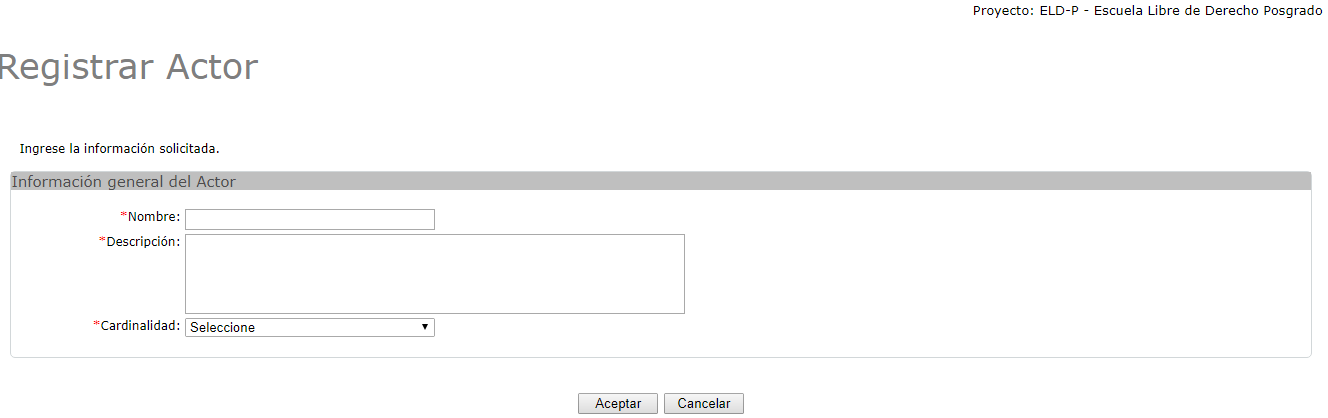
\includegraphics[scale=0.5]{roles/lider/actor/pantallas/IU10-1registrarActor}
					\caption{Registrar Actor}
					\label{fig:registrarActor}
				\end{center}
			\end{figure}
		
			\item Ingrese el nombre, una pequeña descripción y elija el tipo cardinalidad del actor.
			
			\item Oprima el botón \IUAceptar.
			
			\item Se mostrará el mensaje \ref{fig:actorRegistrado} en la pantalla \ref{fig:GestionarActores} ''Gestionar Actores''.
			
			\begin{figure}[htbp!]
				\begin{center}
					
\includegraphics[scale=0.5]{roles/lider/actor/pantallas/IU10-1MSG1}
					\caption{MSG: Actor Registrado}
					\label{fig:actorRegistrado}
				\end{center}
			\end{figure}
			\end{enumerate}